\ifdefined\AuthorVersion
\documentclass[manuscript,screen]{acmart}
\else
\documentclass[manuscript,screen,review,anonymous]{acmart}
\fi
\setcopyright{none}
\settopmatter{printacmref=false}
\acmJournal{DTRAP}
\acmDOI{}
\usepackage{amsmath,booktabs,tabularx,array,graphicx,placeins}
\setlength{\emergencystretch}{2em}
\newcommand{\F}{\textsc{Frozen}}
\newcommand{\FIT}{\textsc{Fit192}}
\newcommand{\CAL}{\textsc{Role64}}
\newcommand{\code}[1]{\texttt{\detokenize{#1}}}
\newcommand{\pp}{\,\mathrm{pp}}
\newcommand{\meanauc}{\overline{\mathrm{AUC}}_{\mathrm{block}}}
\makeatletter
\newcommand{\tablerows}[1]{\@@input #1 }
\makeatother

\renewcommand{\thesection}{S\arabic{section}}
\renewcommand{\thetable}{S\arabic{table}}
\renewcommand{\thefigure}{S\arabic{figure}}
\title{Supplementary Material: Thresholds and Learning in Adaptive Intrusion Detection}
\ifdefined\AuthorVersion\author{Oleksandr Kuznetsov}
\orcid{0000-0003-2331-6326}
\authornote{Corresponding author.}
\email{oleksandr.kuznetsov@uniecampus.it}
\affiliation{\department{Department of Theoretical and Applied Sciences}\institution{eCampus University}\city{Novedrate}\country{Italy}}
\affiliation{\department{SMARTEST Research Center}\institution{eCampus University}\city{Novedrate}\country{Italy}}
\affiliation{\department{Department of Intelligent Software Systems and Technologies, School of Computer Science and Artificial Intelligence}\institution{V. N. Karazin Kharkiv National University}\city{Kharkiv}\country{Ukraine}}
\author{Emanuele Pio De Bernardis}
\orcid{0009-0004-7915-5204}
\email{emanuelepio.debernardis@gmail.com}
\affiliation{\department{Department of Theoretical and Applied Sciences}\institution{eCampus University}\city{Novedrate}\country{Italy}}
\author{Emanuele Frontoni}
\orcid{0000-0002-8893-9244}
\email{emanuele.frontoni@unimc.it}
\affiliation{\department{Department of Political Sciences, Communication and International Relations}\institution{University of Macerata}\streetaddress{Via Crescimbeni, 30/32}\city{Macerata}\postcode{62100}\country{Italy}}
\renewcommand{\shortauthors}{Kuznetsov et al.}
\newcommand{\setauthorpdfmetadata}{\hypersetup{pdfauthor={Oleksandr Kuznetsov; Emanuele Pio De Bernardis; Emanuele Frontoni}}}
\else\author{Anonymous Authors}\fi

\begin{document}
\ccsdesc[500]{Security and privacy~Intrusion detection systems}
\keywords{intrusion detection, threshold selection, calibration coverage, supplementary evidence}
\maketitle
\ifdefined\AuthorVersion\setauthorpdfmetadata\fi
This supplement preserves the historical campaign, its development record, and full diagnostics. All five-seed summaries describe algorithmic randomization conditional on the same recorded stream. Historical measurements and later reconstructions are separate evidence stages. The main article gives the current interpretation; the archived negative and unfavorable results remain available here.
\section{Historical protocol and implementation}
\subsection{Dataset, feature availability, and chronological partitions}
The source network archive contains 22,339,021 rows. The preprocessing manifest records 869 invalid rows and 22,338,152 retained rows. The retained input vector contains eight numerical fields in this order: \code{duration}, \code{src_bytes}, \code{dst_bytes}, \code{missed_bytes}, \code{src_pkts}, \code{src_ip_bytes}, \code{dst_pkts}, and \code{dst_ip_bytes}. Binary labels distinguish normal traffic from attacks. The eight-feature contract was inherited from the project's compact-detector experiments: it uses flow-level numerical aggregates without IP identifiers, ports, application strings, or categorical encodings. Holding it fixed makes the adaptation intervention comparable, but is not a feature-optimality claim. The chronological evaluation stream retains its observed prevalence.

Records are ordered by their complete-feature availability time,
\begin{equation}
 t_{\mathrm{ready}}=t_{\mathrm{start}}+\mathrm{duration}.
 \label{eq:ready}
\end{equation}
This is an offline flow-completion replay. It does not assume that duration or byte totals are known at the first packet. The retained data cover ten UTC calendar days in April 2019, with no retained interval from 5 to 22 April. Table~\ref{tab:data} defines the four chronological partitions. A estimates the initial transformation and model; B selects the initial threshold; C supports development; and D is reserved for the final predictive campaign.

\begin{table}[tb]
\centering\small
\caption{Chronological data partitions. Counts refer to retained rows; normal and attack counts sum to each partition total. The separate overlap strata are described in Section~\ref{sec:overlap}.}
\label{tab:data}
\begin{tabular}{llrrr}
\toprule
Partition & UTC dates, April 2019 & Total & Normal & Attack \\
\midrule
A: initial fit & 2--4, 23 & 3,956,308 & 223,199 & 3,733,109 \\
B: initial threshold & 24 & 5,681,198 & 89,323 & 5,591,875 \\
C: development & 25--26 & 9,150,673 & 173,316 & 8,977,357 \\
D: final evaluation & 27--29 & 3,549,973 & 309,673 & 3,240,300 \\
\bottomrule
\end{tabular}
\end{table}

Attack composition changes across these intervals. A contains scanning attacks; B contains scanning and denial of service. C contains distributed denial of service, denial of service, injection, and password attacks. D contains backdoor, man-in-the-middle, password, ransomware, and cross-site scripting records. These changes provide temporal heterogeneity, but the experiment does not identify a causal type of drift. Backdoor, man-in-the-middle, ransomware, and cross-site scripting are absent from A/B/C; password also occurs in C. The extension reports per-family attack recall.

Before the final campaign, D had been read for structural checks and feature-vector overlap analysis. Its predictive evaluation was run only after the protocol and code were fixed. Accordingly, D is a later evaluation interval, not a completely unseen resource in the broader research process. The five initial models and their B thresholds are prepared before the final runner loads D. C is used in that runner to construct the prior-vector inventory; the C adaptive state is not carried into D.

\subsection{Initial model and restricted adaptation}
Each raw input is transformed by $\log(1+\max(x,0))$ and standardized using means and standard deviations estimated from A. A zero standard deviation is replaced by one. The transformation remains fixed. Each transformed feature is then mapped to its range observed in A and clipped to $[0,1-10^{-9}]$ for spline evaluation. Values outside the observed range therefore saturate at a boundary rather than extrapolating the spline.

For input $j$, the model contains eight cubic B-spline basis functions $B_{jr}$ with an open knot vector based on six equally spaced positions between zero and one. The initial function is
\begin{equation}
 f_j(x_j)=\sum_{r=1}^{8}\theta_{jr}B_{jr}(u_j(x_j)),
 \qquad s(x;g,b)=b+\sum_{j=1}^{8}g_j f_j(x_j).
 \label{eq:model}
\end{equation}
The 64 spline coefficients and initial intercept are fitted by logistic regression on a uniform, seeded 400,000-row sample of A. The implementation uses scikit-learn with \code{C=1.0} and \code{max_iter=1000} \citep{pedregosa2011}. The initial gains are $g_j=1$. Subsequent adaptation leaves the transformation, knots, and all $\theta_{jr}$ fixed, and refits only the eight gains and intercept on the current fitting memory. Each refit solves a new logistic-regression problem with L2 shrinkage of the eight weights toward zero and an unpenalized intercept. It neither starts from nor penalizes distance to the previous head. The fixed spline functions retain information from A, while the head is newly fitted to the current memory. The extension explicitly tests a penalty centred at the previous head.

The empirical object is a logistic generalized additive model with an adaptive linear combination of fixed spline functions. Head refitting can reweight these functions, but cannot learn a new spline shape or an interaction between inputs.

\subsection{Threshold objective and four paired traces}
The implementation predicts attack when $s(x)>\tau$ and normal otherwise. For labeled set $\mathcal{L}$, the threshold objective is
\begin{equation}
 \tau^{*}(\mathcal{L},s)\in\arg\max_{\tau\in\mathcal{T}}
 \frac{1}{2}\left[\frac{\mathrm{TP}(\tau)}{P}+
 \frac{\mathrm{TN}(\tau)}{N}\right],
 \label{eq:threshold}
\end{equation}
where $P$ and $N$ are the attack and normal counts in $\mathcal{L}$. Candidates comprise the distinct observed scores and a floating-point value strictly below the minimum; together with the maximum observed score, this covers the all-attack and all-normal decisions. Scores and objective values use float64. Maximizers are selected by exact equality, without a tolerance, and ties are resolved by the lower median of the sorted maximizing candidates, at zero-based index $\lfloor(m-1)/2\rfloor$. This is a deterministic convention, not a demonstrated threshold-stability property.

The B threshold is selected separately for each initial model using all of B, then kept fixed in the corresponding B traces. Table~\ref{tab:traces} defines the four traces. Both frozen traces use identical initial scores; both FIT192 traces use an identical adapted score trajectory. Consequently, a threshold-only contrast cannot change AUROC. All traces share the same label requests and update eligibility decisions within a seed.

\begin{table}[tb]
\centering\small
\caption{Four paired traces. B denotes the initial fixed threshold; ROLE64 denotes recent threshold selection. The primary contrast is the last row minus the second row.}
\label{tab:traces}
\begin{tabularx}{\linewidth}{lXX}
\toprule
Trace & Score function & Decision threshold \\
\midrule
Frozen / B & Initial A model & Fixed, selected on B \\
Frozen / ROLE64 & Initial A model & Selected on recent ROLE64 labels \\
FIT192 / B & Head refitted on FIT192 & Fixed, selected on B \\
FIT192 / ROLE64 & Same refitted head as FIT192 / B & Selected on recent ROLE64 labels \\
\bottomrule
\end{tabularx}
\end{table}

\subsection{Label budget, delay, and memory separation}
D is divided into 354 blocks of 10,000 records and a final block of 9,973 records, indexed from 0 to 354. Predictions for a block are emitted before any labels from that block enter the controller. A uniform sample without replacement requests $\lfloor0.01 n_k\rfloor$ labels from block $k$: 100 from a full block and 99 from the last block. Requested labels arrive at the end of block $k+1$ and can first influence predictions in block $k+2$ (Figure~\ref{fig:protocol}). Thus 35,499 labels are requested, of which the final 99 remain pending when the observed stream ends. Full labels are available only to the offline evaluation code; the online update receives the delayed requested subset.

\begin{figure}[tb]
\centering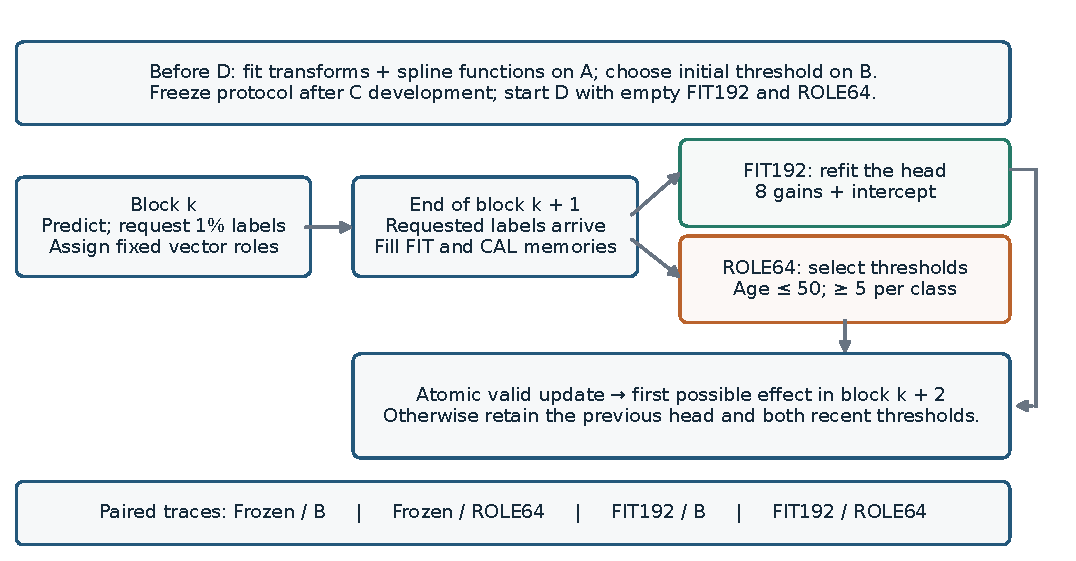
\includegraphics[width=\linewidth]{figures/fig1_protocol.pdf}
\caption{Causal protocol. A label requested in block $k$ cannot affect predictions before block $k+2$. Fitting and threshold selection use separate memories; all state changes are committed together only after the eligibility checks succeed.}
\label{fig:protocol}
\Description{Causal protocol. A label requested in block $k$ cannot affect predictions before block $k+2$. Fitting and threshold selection use separate memories; all state changes are committed together only after the eligibility checks succeed.}
\end{figure}

Both memories start empty at the beginning of D. FIT192 holds at most 192 labeled examples, with target quotas of 96 normal and 96 attack examples. ROLE64 holds at most 64 examples, with target quotas of 32 per class. Either class can borrow unused capacity. On overflow, the oldest example from a class above quota is removed. The quotas alter the stored fitting and threshold-selection samples, not the evaluation stream or the requested-label budget.

A fixed salted SHA-256 rule assigns each raw eight-feature vector permanently to one role: digest modulo four equal to zero selects CAL, and other values select FIT. This prevents an identical vector from appearing in both fitting and calibration memories, even if it recurs later in the stream. It does not deduplicate either memory internally. Role serialization uses canonical float64 bytes; exact overlap between chronological partitions is measured separately using the stored float32 vectors. Appendix~\ref{sec:implementation} specifies these encodings.

FIT192 requires both binary classes. ROLE64 contributes only entries observed at most 50 blocks earlier and requires at least five normal and five attack labels. FIT192 has no corresponding age cutoff. If these conditions hold, the implementation fits a candidate head, scores the eligible ROLE64 examples with both the frozen and candidate heads, and computes two thresholds using Equation~\ref{eq:threshold}. A valid candidate head and both thresholds replace the prior state atomically for the next block. A failed eligibility or numerical check leaves all prior state unchanged and records the reason.

This common schedule isolates the effect of enabling head fitting within the fixed controller, while keeping threshold data and update eligibility matched. It does not estimate a benefit per additional label: FIT192/ROLE64 can use FIT-role labels that Frozen/ROLE64 leaves unused. The extension therefore adds independently eligible ROLE64 and a frozen ALL256 control that can use every acquired label. The 256-example capacity also excludes the delayed-label queue, model state, feature transformations, Python object overhead, temporary solver arrays, and full input arrays used by the offline runner. It must not be interpreted as a total memory bound for an embedded implementation.

\subsection{Overlap-aware reporting}\label{sec:overlap}
The chronological partitions have disjoint row identities, but their eight-feature vectors overlap. An exact SHA-256 inventory of A/B/C marks each D vector as previously observed or unobserved. In D, 37.23\% of rows and 58.03\% of normal rows match a prior vector. The unobserved-vector mask retains 2,228,436 rows: 129,982 normal and 2,098,454 attack observations. The complementary seen stratum contains 179,691 normal and 1,141,846 attack observations.

This mask is applied only when aggregating predictions. It changes neither the prediction sequence nor the adaptive state. Requested labels from all of D can still enter the controller, and repetitions within D remain. The supplementary result therefore measures performance on vectors absent from A/B/C during the same adaptive replay. It is not a separately trained no-overlap experiment, an unseen-attack-family test, or a guarantee that a vector has never previously affected the state within D. A matching eight-feature vector is also not proof that two original network events are duplicates.

\subsection{Metrics, paired seeds, and decision criterion}
We report global false negatives (FN), false positives (FP), attack recall $\mathrm{TP}/P$, false-positive rate $\mathrm{FP}/N$, and balanced accuracy
\begin{equation}
 \mathrm{BA}=\tfrac12\left(\mathrm{recall}+1-\mathrm{FPR}\right).
\end{equation}
These rates are computed from the confusion matrix aggregated over the selected scope. Ranking is summarized by the unweighted mean of AUROC over blocks containing both classes:
\begin{equation}
 \meanauc=\frac{1}{|\mathcal{V}|}\sum_{k\in\mathcal{V}}\mathrm{AUC}_k.
\end{equation}
Undefined AUROCs remain missing. Valid denominators are 352 of 355 blocks for all D and 350 of 355 for the A/B/C-unseen subset. This statistic is not the AUROC obtained by pooling every score across the stream; it does not require scores from different adaptive states to be directly comparable.

Seeds 42--46 determine the initial A subsample and block-level label sampling. The original sampler initializes each block with seed+k; different seed/block pairs can therefore reuse the same relative query positions. The extension replaces this with a tuple-keyed SeedSequence while retaining common requests across methods. Each seed shares all observations and requests across its four traces. Values are means and sample standard deviations ($n-1$ denominator) over the five seeds. Differences are computed within seed before aggregation. These deviations describe stochastic variation conditional on one recorded stream; they are neither confidence intervals nor variation across five independent datasets.

The versioned protocol fixed the primary comparison as FIT192 / ROLE64 minus Frozen / ROLE64. Its decision criterion required $\Delta\mathrm{FN}\leq0$ and $\Delta\mathrm{FP}\leq0$, with at least one strict inequality, in at least four of five seeds. This is a pre-specified empirical acceptance rule, not a statistical significance test or an externally registered trial. The full-stream and supplementary outcomes are reported whether or not the criterion succeeds. We do not select a new operating threshold using final D outcomes.


\FloatBarrier
\section{Historical TON evidence and development record}
\subsection{Development evidence motivating the final comparison}
Development on C proceeded through four recorded stages. These stages answer different questions and are not a single ranking of competing algorithms. In the initial adaptation study, selecting updates using evidence of score inversion outperformed a random schedule with the same number of updates in mean block AUROC by 0.0217, 0.0559, and 0.0719 for logistic regression, an MLP, and the additive spline model, respectively, against the mean of 20 random schedules. For the additive spline model, none of these update policies exceeded the frozen mean block AUROC of 0.8911: evidence-driven, continuous, and random updates attained 0.8341, 0.8073, and 0.7621. The fitted-memory inversion diagnostic was in sample, and out-of-sample evidence from requested block labels was often unavailable or weak after the required delay. Improved ranking did not consistently improve both error counts.

The next stage changed the memory policy while retaining a 256-example capacity. For the continuously updated spline model, class-aware memory increased mean block AUROC by about 0.084 compared with global FIFO, while attack recall fell by 56.66 percentage points at the fixed historical threshold. Subsequent threshold experiments showed why score and decision changes had to be separated. Re-selecting only the frozen spline threshold improved recall on C by 17.73 percentage points and increased FPR by 1.48 percentage points, with exactly unchanged AUROC. Recalibration using the entire B archive was also explored during development, but that configuration required the additional historical archive and is not presented as satisfying the final 256-example online-memory contract.

The final development configuration separated FIT192 and ROLE64. For seed 42 on C, FIT192 / ROLE64 reduced FPR by 16.08 percentage points relative to Frozen / ROLE64, but reduced recall by 2.60 percentage points and mean block AUROC by about 0.109. This mixed outcome motivated preserving the four traces and reporting FN and FP separately in the final evaluation. The C findings are development evidence, not an additional independent confirmation of the final D result.

\subsection{Absolute outcomes on the final interval}
Tables~\ref{tab:rates} and~\ref{tab:counts} report all four traces, including the controls that retain the B threshold. With frozen weights, recent threshold selection raises mean attack recall on all D from $21.11\%$ to $89.09\%$, while FPR rises from $12.64\%$ to $46.74\%$. Mean block AUROC remains $0.8536$ because the scores are identical. Thus, a large recovery in recall can arise entirely from moving the decision threshold.

\begin{table}[tb]
\centering\fontsize{8.6}{10.5}\selectfont
\setlength{\tabcolsep}{4pt}
\caption{Final rates: mean $\pm$ sample SD over five paired seeds. Recall, FPR, and BA are percentages calculated globally. AUROC is the unweighted mean over valid blocks (352/355 for all D; 350/355 for A/B/C-unseen vectors), then averaged over seeds.}
\label{tab:rates}
\begin{tabular}{lrrrr}
\toprule
Trace & Recall (\%) & FPR (\%) & BA (\%) & Mean block AUROC \\
\midrule
\tablerows{tables/rates_rows.tex}
\bottomrule
\end{tabular}
\end{table}

\begin{table}[tb]
\centering\small
\caption{Absolute final error counts: mean $\pm$ sample SD over five seeds. Noninteger means result from averaging integer counts. The paired differences in Table~\ref{tab:paired} retain the seed correspondence.}
\label{tab:counts}
\begin{tabular}{lrr}
\toprule
Trace & False negatives & False positives \\
\midrule
\tablerows{tables/counts_rows.tex}
\bottomrule
\end{tabular}
\end{table}

The FIT192/B diagnostic displays the expected risk of retaining a threshold after changing the fitted sample and score scale. FIT192 / B reaches mean block AUROC $0.9359$, yet attack recall is only $8.81\%$ and FPR is $0.88\%$. The ranking improves on average, but the inherited threshold misses most attacks. Refitting with approximately balanced class quotas differs from fitting A, where about 94\% of observations are attacks. Under pure prior shift, the log-odds correction would be an intercept shift; here reweighted slopes and changing class-conditional traffic also contribute. Thus this control illustrates score--threshold mismatch rather than a newly discovered property of logistic models. With the same adapted scores and a recent threshold, FIT192 / ROLE64 reaches recall $89.38\%$ and FPR $20.47\%$. Relative to FIT192 / B, this threshold change removes 2,610,759.8 mean false negatives at the cost of 60,637.6 additional false positives. Figure~\ref{fig:operating} shows the resulting operating-point changes.

\begin{figure}[tb]
\centering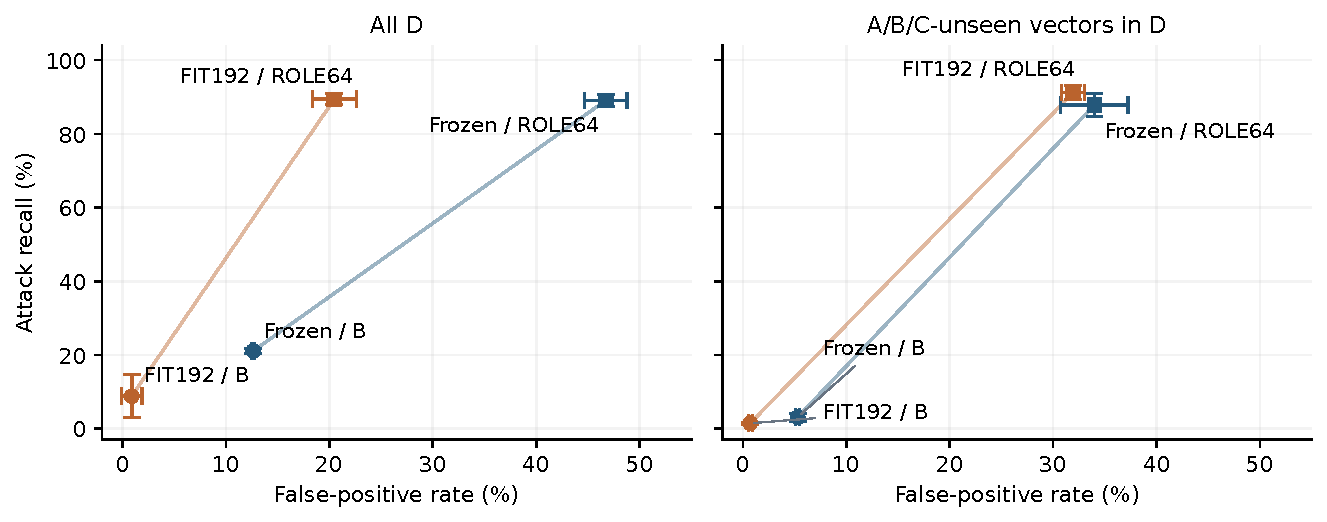
\includegraphics[width=\linewidth]{figures/fig2_operating_points.pdf}
\caption{Operating points on the same final replay. Points are seed means; bars show sample SD. Lines connect traces with identical score functions and different threshold policies, not a continuously optimized ROC curve. The large threshold effects coexist with a narrower primary comparison between the two ROLE64 traces.}
\label{fig:operating}
\Description{Operating points on the same final replay. Points are seed means; bars show sample SD. Lines connect traces with identical score functions and different threshold policies, not a continuously optimized ROC curve. The large threshold effects coexist with a narrower primary comparison between the two ROLE64 traces.}
\end{figure}

\subsection{Primary paired comparison and the joint-error criterion}
The primary contrast compares FIT192 / ROLE64 with Frozen / ROLE64. On all D, mean balanced accuracy improves by $13.28\pm2.26$ percentage points and mean block AUROC by $0.0823\pm0.0155$. Mean FP decreases by $81{,}355.4\pm6{,}051.6$. Mean FN decreases by $9{,}255.2\pm97{,}413.0$, corresponding to a recall difference of $0.29\pm3.01$ percentage points. Hence the average balanced-accuracy gain is predominantly associated with lower false-positive rates, while the missed-attack outcome is variable.

The per-seed counts in Table~\ref{tab:paired} and Figure~\ref{fig:paired} show the limitation directly. All five seeds reduce FP on the full stream, but seeds 42 and 44 increase FN. Seeds 43, 45, and 46 improve both counts. The pre-specified four-of-five criterion is therefore not met. The sign of the mean FN change does not overturn that result, and the sample SD should not be read as a confidence bound supporting superiority.

\begin{table}[tb]
\centering\small
\caption{Primary paired differences, FIT192 / ROLE64 minus Frozen / ROLE64. Negative values indicate fewer errors. Seeds 43, 45, and 46 jointly improve FN and FP in both reporting scopes; seed 44 worsens both on A/B/C-unseen vectors.}
\label{tab:paired}
\begin{tabular}{crrrr}
\toprule
 & \multicolumn{2}{c}{All D} & \multicolumn{2}{c}{A/B/C-unseen vectors} \\
\cmidrule(lr){2-3}\cmidrule(lr){4-5}
Seed & $\Delta$FN & $\Delta$FP & $\Delta$FN & $\Delta$FP \\
\midrule
\tablerows{tables/paired_rows.tex}
\bottomrule
\end{tabular}
\end{table}

\begin{figure}[tb]
\centering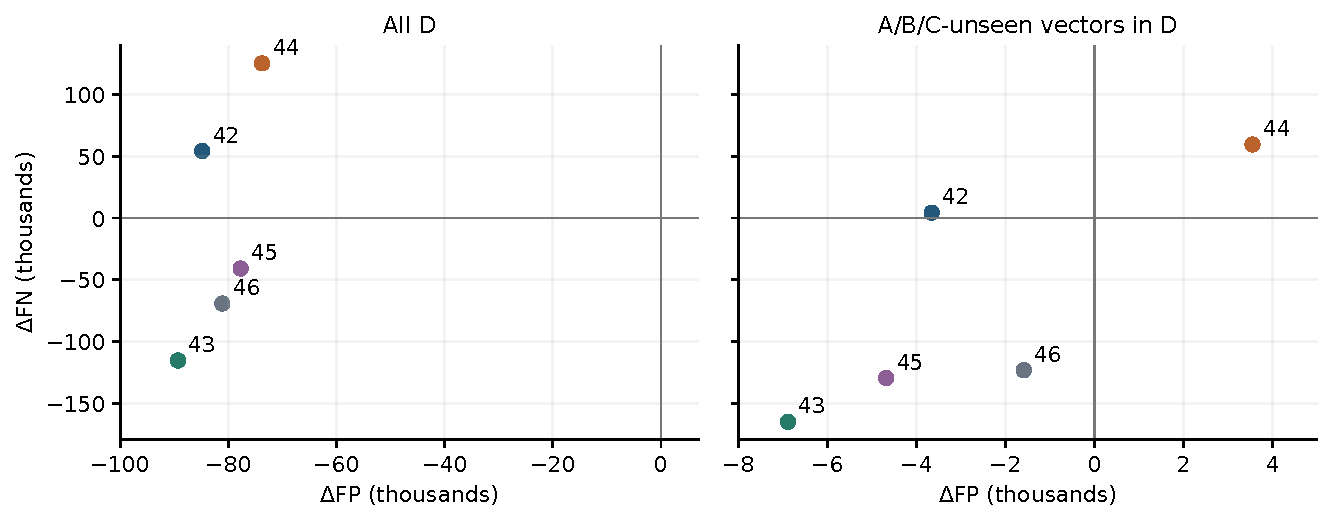
\includegraphics[width=\linewidth]{figures/fig3_paired_deltas.pdf}
\caption{Primary paired differences by seed. Both axes show thousands of errors. Joint improvement requires a point in the lower-left quadrant (including a non-deteriorating boundary). The horizontal scales differ to make the much smaller unseen-vector FP changes visible.}
\label{fig:paired}
\Description{Primary paired differences by seed. Both axes show thousands of errors. Joint improvement requires a point in the lower-left quadrant (including a non-deteriorating boundary). The horizontal scales differ to make the much smaller unseen-vector FP changes visible.}
\end{figure}

\subsection{Previously unobserved vectors and concentration of the FP gain}
For D vectors absent from A/B/C, FIT192 / ROLE64 reaches $91.20\%$ attack recall but an FPR of $31.94\%$. The corresponding Frozen / ROLE64 rates are $87.83\%$ and $33.99\%$. The paired BA gain is $2.71\pm3.63$ percentage points, substantially smaller than the full-stream gain. Mean FN decreases by $70{,}828.6\pm97{,}060.6$ and mean FP by $2{,}655.2\pm3{,}957.2$. Again, only three of five seeds jointly improve both counts.

\begin{table}[tb]
\centering\small
\caption{Complementary overlap strata in the original campaign: mean $\pm$ seed SD. Rates are percentages. The same adaptive trajectory supplies both strata.}
\label{tab:strata}
\begin{tabular}{llrrr}
\toprule
Stratum & Trace & Recall & FPR & BA \\
\midrule
\tablerows{tables/strata_rows.tex}
\bottomrule
\end{tabular}
\end{table}

The complementary seen stratum exposes the trade-off (Table~\ref{tab:strata}). Head adaptation lowers recall from 91.41\% to 86.02\%, while FPR falls from 55.96\% to 12.16\%. It adds 61,573.4 mean FN while removing 78,700.2 FP. In the unseen stratum it removes 70,828.6 FN and 2,655.2 FP. Thus the small full-stream mean FN reduction combines effects with opposite signs. The seen stratum contributes 96.7\% of the total FP reduction, but that percentage describes the location of FP savings rather than the fraction of all benefit caused by overlap. The strata differ in traffic composition and share one adaptive state.

The factorial BA interaction is positive in every original full-stream seed: 10.76--17.65 percentage points, with mean 13.55. On unseen vectors it ranges from $-4.43$ to $+4.89$ points, with mean 1.24. The gain from jointly changing the head and threshold therefore depends on the reporting population. The four-trace interaction and the complementary-stratum decomposition reveal information concealed by a single average BA gain.

\subsection{When limited labels prevent adaptation}
Label availability creates a distinct temporal failure mode in the C development replay. There are 440 skipped update decisions, all associated with insufficient recent normal examples for calibration. The longest consecutive sequence spans decision blocks 241--663 and affects predictions in blocks 242--664: 423 blocks. Figure~\ref{fig:gating} shows the eligible normal-label count and the corresponding decision rates.

\begin{figure}[tb]
\centering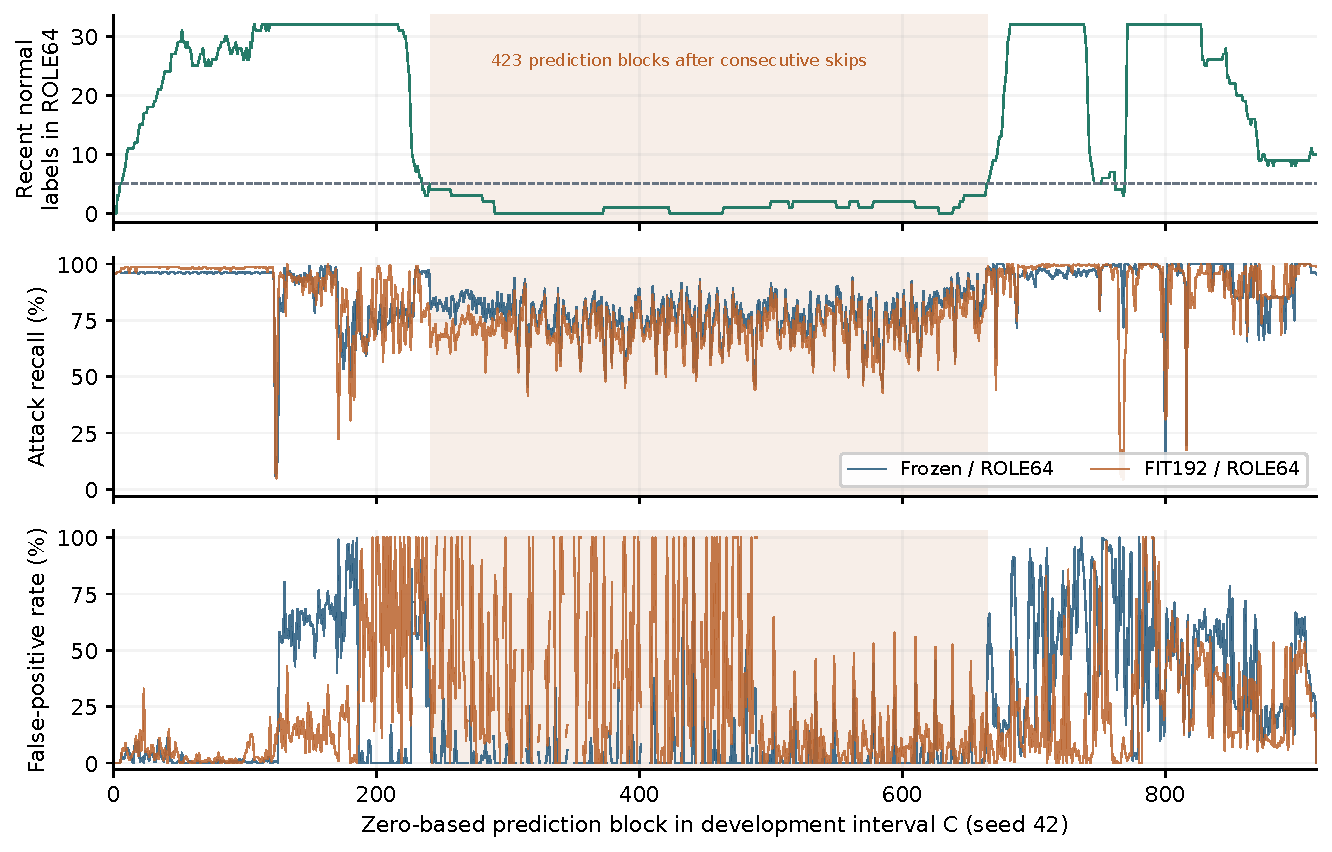
\includegraphics[width=\linewidth]{figures/fig4_development_gating.pdf}
\caption{Development interval C, seed 42. Shading marks prediction blocks 242--664, following 423 consecutive skipped update decisions. The upper panel shows the recorded number of recent normal examples in ROLE64, with the minimum of five indicated. Recall and FPR are per-block values; undefined class-specific rates remain gaps. The display is descriptive and does not randomize the occurrence of skips.}
\label{fig:gating}
\Description{Development interval C, seed 42. Shading marks prediction blocks 242--664, following 423 consecutive skipped update decisions. The upper panel shows the recorded number of recent normal examples in ROLE64, with the minimum of five indicated. Recall and FPR are per-block values; undefined class-specific rates remain gaps. The display is descriptive and does not randomize the occurrence of skips.}
\end{figure}

Stratifying predictions by the preceding update decision yields opposite FN patterns. Across 474 blocks following applied updates, FIT192 / ROLE64 has 29,697 fewer FN and 26,528 fewer FP than Frozen / ROLE64. Across 440 blocks following skips, it has 263,032 more FN and 1,342 fewer FP. In the longest skipped segment alone, both counts worsen: FN increases by 219,608 and FP by 807. These are post hoc associations conditioned on the realized stream. The segments have different class composition and cannot establish that skipping caused the deterioration.

The final D replay behaves differently. Of 354 recorded update opportunities per seed, 337, 351, 347, 341, and 350 are accepted for seeds 42--46, respectively. Their 17, 3, 7, 13, and 4 skips all occur before the first valid update. There is no recurrence of the long post-update starvation interval observed on C. The historical D record shows a different eligibility pattern from development C.

\subsection{Measured computation and its boundary}
Table~\ref{tab:cost} gives recorded computational costs on the original evaluation machine: Windows 11, Python 3.13.2, NumPy 2.3.4, scikit-learn 1.7.2, an Intel processor reported as Family 6 Model 186 Stepping 3, 12 visible CPU threads, and 16,067.4 MiB of system RAM. These are elapsed times from one execution environment, not cross-device benchmarks.

\begin{table}[tb]
\centering\small\setlength{\tabcolsep}{4.5pt}
\caption{Recorded final-run costs in seconds. Fits and threshold-selection times are components included within replay time, not extra times to add to it. The final recorded update has no subsequent evaluated block.}
\label{tab:cost}
\begin{tabular}{crrrrrr}
\toprule
Seed & Updates & Skips & Head fit & Frozen threshold & Adapted threshold & D replay \\
\midrule
\tablerows{tables/cost_rows.tex}
\bottomrule
\end{tabular}
\end{table}

The five-seed command takes 1,234.388 seconds within its recorded timer boundary. This includes D hashing and loading, initial A fitting and B preparation, the five D replays, and writing the five per-seed reports. It excludes the earlier A/B/C hash calculation and final summary serialization. Within each replay, accumulated head-fitting time is 9.630--10.672 seconds; each of the two accumulated threshold-selection components is below 0.11 seconds. These observations support only the relative cost of these implementation components in this run. They do not establish an energy advantage, a device-level latency guarantee, or an embedded memory footprint.
\FloatBarrier


\FloatBarrier
\section{Implementation details and reproducibility map}
\label{sec:implementation}
\subsection{Immutable roles and retained examples}
The role hash is SHA-256 over the ASCII salt \code{ADAPT04-C-seed42-v1}, a zero byte, and the eight raw feature values encoded as little-endian float64. Both signs of zero are normalized to positive zero; NaNs are canonicalized. The digest is interpreted as a big-endian integer and assigned to CAL if its remainder modulo four is zero, otherwise to FIT. The salt's historical seed label is literal: the same salt is used for every final seed. Each requested observation retains its assigned role. Stored model inputs are transformed only when its label arrives; the role digest continues to identify the raw vector.

For chronological overlap, the separately defined fingerprint is SHA-256 over the 32 bytes of the eight stored float32 inputs in little-endian order. This predicate checks equality at the stored feature precision. It is not an event-identity test. The two hashing procedures have different purposes and must not be substituted for one another in reproduction.

Calibration age is measured from the observation block, not from the arrival block. Repeated vectors can occupy multiple positions in a role memory; the five-per-class minimum counts observations, not unique vectors. Class quotas determine eviction when capacity is exceeded; one class may borrow slots not occupied by the other class. They are not hard per-class maxima, and an age filter determines which retained ROLE64 entries are eligible for threshold selection. FIT192 has no age filter. Pending requests are maintained separately from both memories.

\subsection{Ordering and end-of-stream accounting}
For each block, the runner (i) transforms and scores records using the incoming state, (ii) records the four decision outcomes for the evaluator, (iii) requests labels without using their values, (iv) receives the previous block's requested labels, (v) updates memories, and (vi) attempts an atomic transaction for the next block. Labels from a predicted block do not affect any predictions within that block.

There are 355 prediction blocks but 354 update opportunities because no requested labels arrive at the end of block zero. A decision at the end of the final block is recorded and timed, although its resulting state has no subsequent evaluated block. The last 99 requested labels remain pending. This boundary explains why counts of decisions and counts of affected prediction blocks differ. Likewise, the C temporal stratification excludes the two initial prediction blocks without a preceding delayed-label decision.

\subsection{Artifact entry points}
The following paths are relative to \code{adattamento-drift/ton_temporal/} in the repository snapshot. They provide a direct map from the manuscript to implementation and evidence:
\begin{itemize}\raggedright
\item \code{replay.py}: fixed transformation, additive spline model, logistic head refitting, sampling, and class-aware memory.
\item \code{soglia_bilanciata.py}: strict-threshold convention, candidate construction, exact comparison, and lower-median tie rule.
\item \code{calibrazione_recente.py}: immutable roles, recent-label eligibility, and atomic transaction.
\item \code{replay_validazione_finale.py}: five-seed final replay, paired traces, overlap mask, and aggregate metric definitions.
\item \code{split_manifest.json} and \code{sovrapposizioni_abcd.json}: chronology, counts, historical exposure, and cross-partition vector checks.
\item \code{articolo_02/protocollo_validazione_finale.md}: protocol fixed before the final predictive campaign.
\item \code{articolo_02/validazione_finale_D/analisi_finale.json}: absolute metrics, paired differences, temporal summaries, and measured costs.
\item \path{adapt04_calibrazione_recente/replay_completo/confronto_per_blocco.csv}: C per-block evidence used in Figure~\ref{fig:gating}.
\end{itemize}
The reproduction package retains the original numerical summaries, complete reports and model artifacts described in Section~\ref{sec:extras}. Rebuilding figures is separate from reconstructing raw data and rerunning the predictive campaign.


\FloatBarrier
\section{Diagnostic set A: operating policies and model audits}
\label{sec:diagnostic_a}
The diagnostic protocol was fixed before execution, after all first-extension outcomes were known. It defines 120 predictive cells: 80 spline cells (eight settings, two captures, five seeds), ten LR main cells, and 30 forest cells (three conditions, two captures, five seeds). Thirty main cells repeat previous trajectories to check the new runner. They are not additional independent evidence. The first diagnostic attempt was invalidated after a uint8 overflow was found in the guard that determines whether AP is defined. The retained AP diagnostics use the widened integer-count fix and are checked against AUC class-validity coverage, with a dedicated regression test. This affected the new AP diagnostic only; the historical and first-extension reports remain unchanged. The excluded attempt is identified in the provenance log.

\subsection{Operating-point comparisons}
Retrospective interpolation uses observed FPR/recall points within each seed's support. It uses no extrapolation. FPR ties retain the larger recall for a matched-FPR description; recall ties retain the smaller FPR for a matched-recall description. The result is a piecewise-linear description of recorded policies, not an estimated deployment frontier. The CSV includes missing comparisons when a target is outside either controller's observed support. Averaging paired interpolations differs from interpolating seed means because the operating-point locations vary across seeds.
\begin{table}[htbp]\centering\fontsize{8}{10}\selectfont\setlength{\tabcolsep}{3pt}
\caption{Descriptive matched-FPR comparison of the original five cost points on TON D. The paired columns interpolate within each seed, then summarize the supported pairs. Mean-curve columns interpolate curves of seed means. Values are recall percentages; the difference is in percentage points. No comparison extrapolates.}
\begin{tabular}{rrrrrrr}\toprule
FPR & Pairs & Paired frozen & Paired head & Paired difference & Mean-curve frozen & Mean-curve head \\\midrule
\tablerows{tables/diagnostic_a_matched_rows.tex}\bottomrule\end{tabular}\end{table}
The mean-curve and paired-seed summaries describe different operations. At 13\% FPR, the paired head-minus-frozen difference is $2.41\pm3.11$ percentage points on this stream, whereas the mean curves nearly coincide. These descriptive calculations do not establish equivalence or superiority in a new stream. The low-FPR comparison has incomplete common support. The denser nine-weight audit is retained as additional operating points, without selecting a weight from D for deployment.

With the denser nine-weight grid, the paired head-minus-frozen recall difference at 13\% FPR is $1.49 \pm 3.66$ percentage points (5 supported pairs). This remains a retrospective interpolation within each seed, rather than a threshold selected for a new stream.


\subsection{Model audit and threshold transfer}
Model audits verify that label one denotes an attack and higher scores denote greater attack confidence. LR coefficients, decision-function output, and the attack-probability column are checked directly. Cached D scores are checked on 5,000 fixed sampled observations against direct model predictions. Full A/B/D fixed-score metrics and class-specific score quantiles are retained. A metrics describe the training population, not generalization. Chronological ARF initial fitting and its shuffled control use exactly the same sampled row set; only their order changes.

The fixed LR class ordering is $[0,1]$. Coefficient scores and the attack-probability column agree numerically with the cached score; the full audit records the maximum discrepancies and solver iteration counts. On TON the inversion is already visible on B, before D. This supports poor temporal transfer within the compact feature contract, rather than an implementation that systematically reverses the attack label.

For frozen spline thresholds, the following summaries weight each calibration/next-block pair by the next block's normal count and exclude the initial period before valid calibration. TON, $\lambda=1$: calibration FPR 42.67\%, next-block FPR 48.30\%; median distinct normal scores 55. TON, $\lambda=2$: calibration FPR 8.26\%, next-block FPR 13.20\%; median distinct normal scores 55. UNSW, $\lambda=1$: calibration FPR 2.67\%, next-block FPR 5.64\%; median distinct normal scores 110. UNSW, $\lambda=2$: calibration FPR 2.36\%, next-block FPR 5.16\%; median distinct normal scores 110. The calibration and future populations differ; these are descriptive transfer diagnostics, not estimates of independent calibration-sample uncertainty. Distinct scores can be much fewer than retained normal observations.


\subsection{Conditional ranking and precision--recall summaries}
AP is noninterpolated average precision. AP is recorded for the main, shuffled, and FIT-only conditions; the seven spline sensitivity conditions retain AUC and confusion counts. Blocks containing only one class are excluded from within-block AUC/AP summaries; their counts and class coverage are explicit in the CSV. Macro AP is not pooled AP, and weighting block AP by class counts does not turn it into pooled AP. Precision at each operating policy is computed from globally summed confusion counts. Comparisons across captures must account for their different prevalence.
\begin{table}[htbp]\centering\fontsize{7.5}{9.5}\selectfont\setlength{\tabcolsep}{3pt}
\caption{Ranking summaries, mean $\pm$ seed SD conditional on each capture. NW and AW denote normal-count and attack-count weighting of valid blocks. Adaptive rows use the chronological initialization and default controller.}
\begin{tabular}{lllrrrrr}\toprule
Stream & Model & Score & AUC macro & AUC NW & AP macro & AP NW & AP AW \\\midrule
\tablerows{tables/diagnostic_a_ranking_rows.tex}
\bottomrule\end{tabular}\end{table}

\subsection{Forest feedback and persistent state}
\begin{table}[htbp]\centering\small\setlength{\tabcolsep}{4pt}
\caption{Forest label and state ledger, mean $\pm$ SD conditional on each capture. Learned labels count D arrivals used once for learning, excluding initial A fitting. Final serialized model size excludes external controller memory and is not peak RAM.}
\begin{tabular}{llrrr}\toprule Stream & Condition & Acquired labels & Learned labels & Final model MiB \\\midrule
\tablerows{tables/diagnostic_a_forest_ledger_rows.tex}\bottomrule\end{tabular}\end{table}
Standard and shuffled forests reuse CAL-role labels for learning. The FIT-only condition excludes those labels throughout D, while retaining the same chronological initial state. The acquired budget remains shared even though fewer labels enter learning. Per-seed timings are retained in the CSV; runs execute concurrently, so those timings are audit records rather than a controlled hardware benchmark.

\subsection{Memory, age, eligibility, and role-salt sensitivity}
One factor changes at a time. The default is FIT192/ROLE64, age 50, minimum five CAL observations per class, and salt \code{ADAPT04-C-seed42-v1}. Labels continue to arrive after prediction, and all configurations use the same query sequence for each dataset/seed. The age factor also applies to the independent ALL256 control. FIT entries have no age filter. Capacity variants preserve the nominal 3:1 FIT/CAL allocation but change the total retained examples to 128 or 512. Alternative salt UTF-8 byte strings, encoded here in hexadecimal, are the recorded source revision and the recorded source revision; the same alternative is used for all five seeds. No setting is chosen as a new primary configuration from D results.
\begin{table}[htbp]\centering\small\setlength{\tabcolsep}{4pt}
\caption{Spline head/CAL sensitivity. Rates are percentages, mean $\pm$ sample SD conditional on each stream. Updates are mean valid transactions. Main denotes the default.}
\begin{tabular}{llrrrr}\toprule
Stream & Changed setting & Recall & FPR & BA & Updates \\\midrule
\tablerows{tables/diagnostic_a_sensitivity_rows.tex}
\bottomrule\end{tabular}\end{table}

\subsection{Complete first-extension default comparisons}
The following tables retain all displayed default model comparisons from the first extension. Each seed describes the same captured stream. Frozen LR and chronological ARF quality must be interpreted using the audits in the main paper; the macro AUROC column is accompanied by normal-weighted and pooled summaries elsewhere in this Supplement.
\begin{table}[htbp]\centering\fontsize{8.8}{10.5}\selectfont\setlength{\tabcolsep}{4pt}
\caption{TON first-extension defaults. Rates are percentages, mean $\pm$ SD conditional on one stream; AUROC is the macro mean over valid prediction blocks.}
\begin{tabular}{lrrrr}\toprule Controller & Recall & FPR & BA & AUROC \\\midrule
\tablerows{tables/ton_extension_rows.tex}\bottomrule\end{tabular}\end{table}
\begin{table}[htbp]\centering\fontsize{8.8}{10.5}\selectfont\setlength{\tabcolsep}{4pt}
\caption{UNSW first-extension defaults, with the same conditional reporting convention.}
\begin{tabular}{lrrrr}\toprule Controller & Recall & FPR & BA & AUROC \\\midrule
\tablerows{tables/unsw_extension_rows.tex}\bottomrule\end{tabular}\end{table}
\begin{figure}[htbp]\centering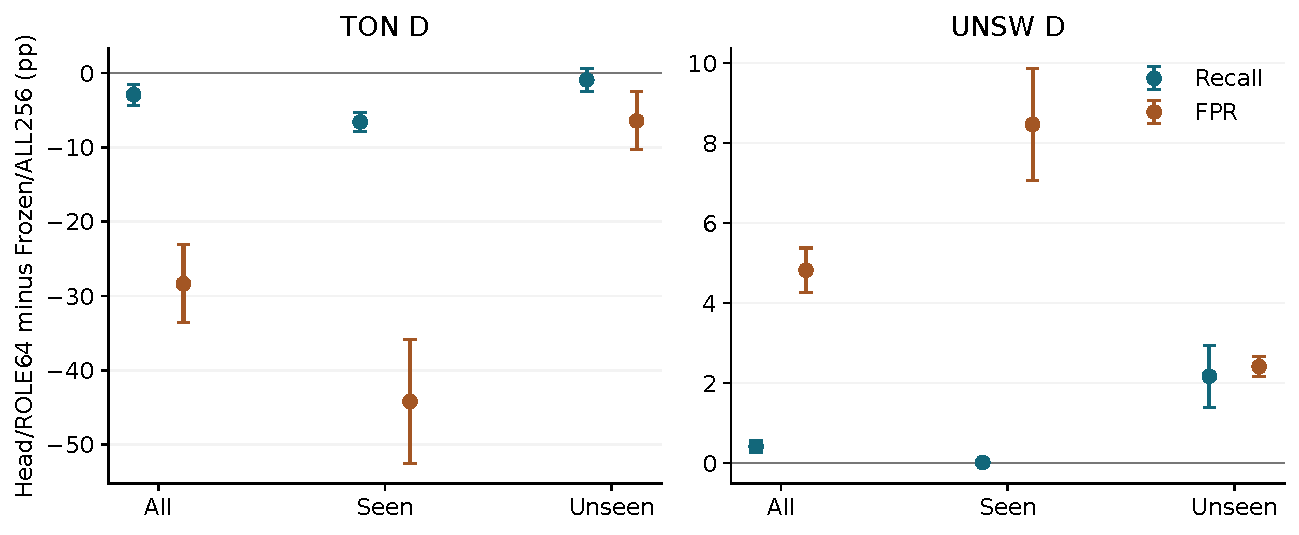
\includegraphics[width=\linewidth]{figures/fig6_stratum_effects.pdf}
\caption{Spline head/ROLE64 minus Frozen/ALL256 at $\lambda=1$ in the first extension, by representation-recurrence stratum. Points are paired seed means and bars are sample SD on the same stream. Positive recall and negative FPR changes favor the head; concurrent reductions describe fewer false alarms at the expense of recall.}
\Description{Spline head/ROLE64 minus Frozen/ALL256 at $\lambda=1$ in the first extension, by representation-recurrence stratum. Points are paired seed means and bars are sample SD on the same stream. Positive recall and negative FPR changes favor the head; concurrent reductions describe fewer false alarms at the expense of recall.}
\end{figure}
\FloatBarrier
\subsection{Additional first-extension controls}
\begin{table}[htbp]\centering\small\setlength{\tabcolsep}{4pt}
\caption{Independent ROLE64, offset-only and prior-centred spline controls. Mean $\pm$ SD describes five randomizations on one stream.}
\begin{tabular}{llrrr}\toprule Dataset & Controller & Recall & FPR & BA \\\midrule
\tablerows{tables/ablation_rows.tex}\bottomrule\end{tabular}\end{table}
Independent ROLE64 produces the same outcomes as the matched ROLE64 schedule in these main runs. Offset/ROLE64 produces the same decisions as frozen/ROLE64, as expected from $s+c>\tau+c$ being equivalent to $s>\tau$. The prior-centred refit minimizes summed logistic loss plus $\tfrac12\lVert w-w_{\rm previous}\rVert^2$, with an unpenalized intercept. Its BA is 84.42\% on TON and 93.72\% on UNSW, compared with 84.84\% and 93.22\% for the default head. It supplies no uniform remedy across the two captures.
\begin{table}[htbp]\centering\fontsize{8.5}{10}\selectfont\setlength{\tabcolsep}{3.4pt}
\caption{First-extension TON delay and budget sensitivity, conditional on the same stream. Default budget is 1\%; only the final pair uses 0.1\%. Updates include the final transaction without a subsequent evaluated block.}
\begin{tabular}{llrrrr}\toprule Condition & Controller & Recall & FPR & BA & Updates \\\midrule
\tablerows{tables/sensitivity_rows.tex}\bottomrule\end{tabular}\end{table}
\FloatBarrier

\FloatBarrier
\section{Supplementary experimental summaries}
\label{sec:extras}
\begin{table}[htbp]
\centering\fontsize{7.8}{9.5}\selectfont\setlength{\tabcolsep}{3pt}
\caption{Extension resource ledger, mean $\pm$ seed SD. Times are seconds. Initial artifact size includes the transform; final base-model size excludes it and all external controller state. Neither size is peak RAM. Offline cached replay is not deployment latency.}
\label{tab:resources}
\begin{tabular}{llrrrrrr}
\toprule
Dataset & Model & Initial fit & B scoring & D cache & Replay & Initial KiB & Final base KiB \\
\midrule
\tablerows{tables/resource_rows.tex}
\bottomrule
\end{tabular}
\end{table}
\begin{table}[htbp]
\centering\small
\caption{Fixed-score ranking summaries in the extension, mean $\pm$ seed SD. Pooled AUROC compares all fixed scores; macro block AUROC weights valid blocks equally; normal-weighted AUROC weights them by normal observations. The full CSV includes valid-block counts and all overlap strata.}
\label{tab:aucsupp}
\begin{tabular}{llrrr}
\toprule
Dataset & Initial model & Pooled AUROC & Macro block & Normal-weighted block \\
\midrule
\tablerows{tables/auc_rows.tex}
\bottomrule
\end{tabular}
\end{table}

\begin{table}[htbp]
\centering\fontsize{8.5}{10}\selectfont\setlength{\tabcolsep}{3.5pt}
\caption{Attack-family recall (percent) for the spline detector in the extension. Counts are evaluated attacks, shared by every trace and seed. Means and sample SDs refer to five seeds. The machine-readable supplement includes LR and ARF, each seed, and every operating-cost policy.}
\label{tab:attacksupp}
\begin{tabular}{llrrrr}
\toprule
Dataset & Attack family & Count & Frozen/B & Frozen/ALL256 & FIT192/ROLE64 \\
\midrule
\tablerows{tables/attack_rows.tex}
\bottomrule
\end{tabular}
\end{table}

\begin{table}[htbp]
\centering\small
\caption{Descriptive moving-block sensitivity of the original paired FIT192/ROLE64 minus Frozen/ROLE64 errors. Brackets are 2.5th--97.5th resampling percentiles, not confidence intervals for a refitted adaptive process. Each analysis resamples contiguous blocks of the recorded error trajectories, sharing block selections across seeds and policies.}
\label{tab:bootsupp}
\begin{tabular}{lrrrr}
\toprule
Scope & Block length & $\Delta$FN (thousands) & $\Delta$FP (thousands) & $\Delta$BA (pp) \\
\midrule
\tablerows{tables/bootstrap_rows.tex}
\bottomrule
\end{tabular}
\end{table}

For the resampling lengths in Table~\ref{tab:bootsupp}, the full-stream FN range crosses zero while the FP range remains negative. On unseen vectors the FP and BA ranges cross zero. This reinforces the distinction between an aggregate FP saving and stable joint improvement, but the ranges are conditional summaries of the recorded trajectories. A valid inference about retrained policies under a new process would require a sampling design for that process and rerunning the adaptive state transitions.

\subsection{Numerical bridge and archive contents}
The legacy-sampler reruns use exactly the original requested row identities in every block. Their mean FIT192/ROLE64 outcomes are close to the original aggregates (the FN difference is $-563.0$ and the FP difference is $-7.4$), but individual seeds and some other traces differ materially. For example, the FIT192/B FN difference ranges from $-9{,}617$ to $+335{,}381$. Accordingly, the original per-seed observations and the newly fitted observations are separate evidence stages. The file \path{analysis/legacy_replication_bridge.csv} gives every difference; no rerun is presented as bitwise replication.

The original A parser and the extension A parser produce identical arrays and an identical NPZ file in the present environment. The extension also records array-level digests to distinguish data identity from archive-container bytes. Repeating the initial seed-42 fit with NumPy 2.3.4 and SciPy 1.16.3 in Linux gives the same fitted head as the new environment, so library version labels alone do not identify the source of the Windows/Linux difference. An exact causal attribution would require the original arrays and fitted model state. This residual reproducibility boundary is retained rather than explained speculatively.

The reproduction archive includes all 55 extension reports, the original five full reports, compact fitted initial-model artifacts, input manifests, and a validation summary. \path{analysis/per_seed_metrics.csv} contains every controller, seed, condition, and overlap stratum; \path{analysis/paired_differences.csv} preserves paired comparisons. \path{analysis/attack_family_recall.csv}, \path{analysis/resources_and_labels.csv}, and \path{analysis/time_partitions.json} document attack counts, computational components, feedback timing, and chronology. All paper figures and generated tables can be rebuilt from these artifacts without downloading the raw CSVs.

\FloatBarrier
\section{Diagnostic set B: matched calibration memory}
\label{sec:matchedsupp}
The matched-memory follow-up contains ten additional spline replays: two captures and seeds 42--46. Its protocol and runner were committed before their full executions, after the earlier results and concerns about unequal calibration memory had been examined. It is exploratory on both captures. The larger disjoint ROLE256 buffer receives the same CAL-role arrivals as ROLE64, preserves the original class-eviction rule with borrowing of unused slots, and applies the same 50-block age filter. Occurrence-level nesting of the small buffer inside the large one and FIT/CAL digest disjointness are checked at every arrival. All four thresholds use the successful original FIT192/ROLE64 transaction gate, so the score trajectory and its timing are identical across calibration capacities.

\begin{figure}[tb]
\centering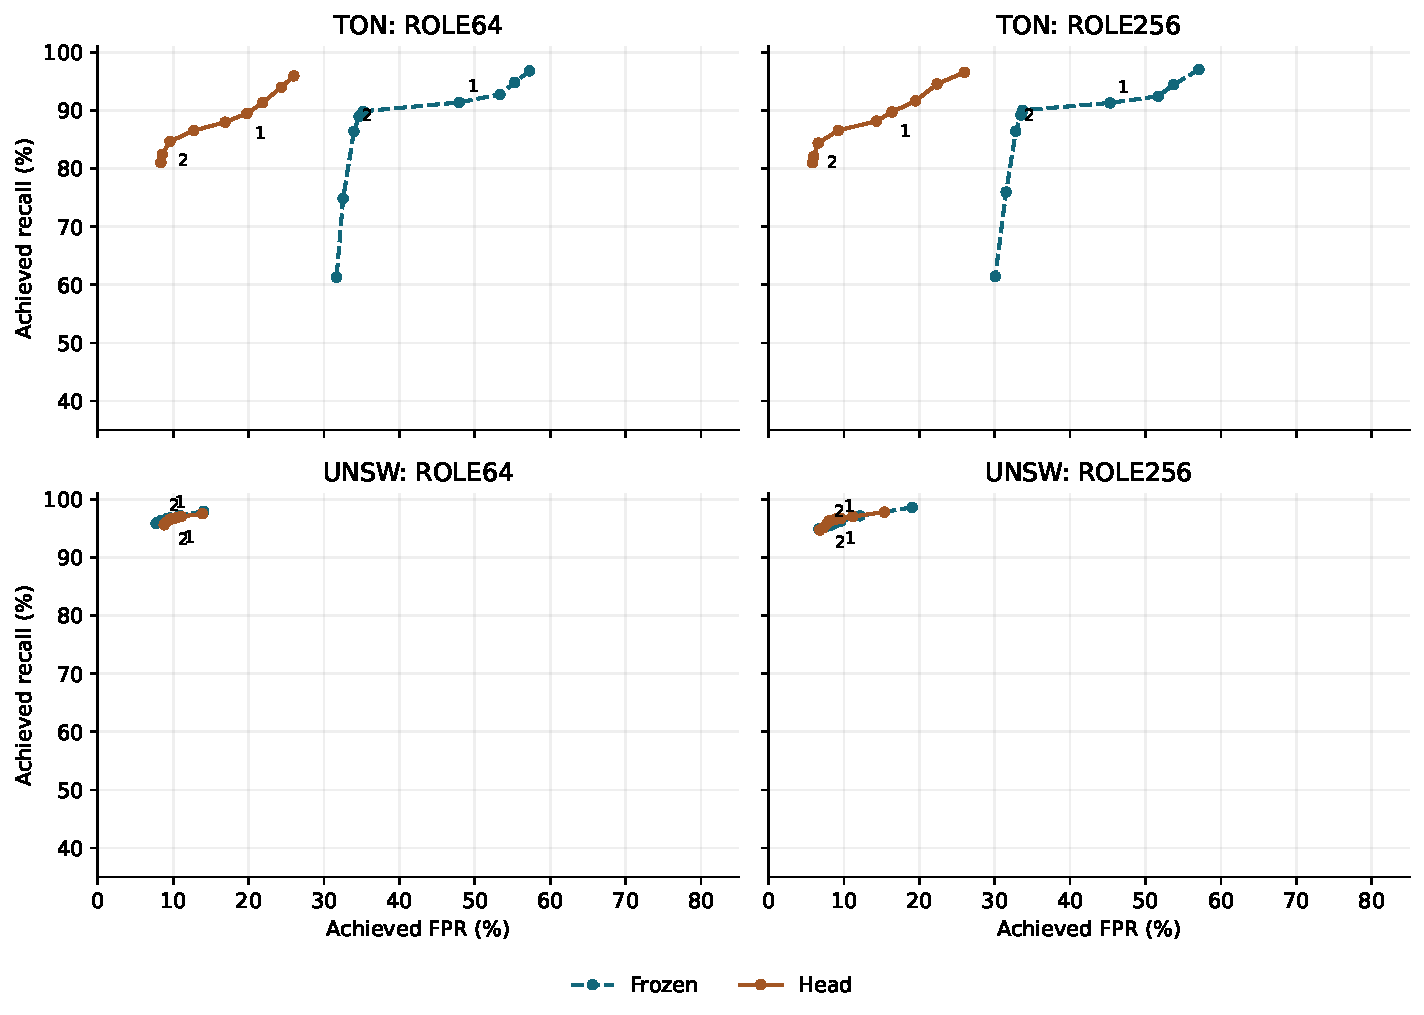
\includegraphics[width=.94\linewidth]{figures/diagnostic_b_same_memory.pdf}
\caption{Same-memory score comparisons, with identical axes in all panels. Within a panel, frozen and head scores use the same calibration occurrences and update times; the head trajectory also stays fixed across columns. The nine cost weights generate causal operating policies, connected in cost-weight order. Numerals mark $\lambda=1$ and 2. Points are means across five randomizations conditional on one capture, not a deployable oracle frontier.}
\Description{Same-memory score comparisons, with identical axes in all panels. Within a panel, frozen and head scores use the same calibration occurrences and update times; the head trajectory also stays fixed across columns. The nine cost weights generate causal operating policies, connected in cost-weight order. Numerals mark $\lambda=1$ and 2. Points are means across five randomizations conditional on one capture, not a deployable oracle frontier.}
\end{figure}

\begin{table}[tb]
\centering\fontsize{9}{10.5}\selectfont\setlength{\tabcolsep}{2.4pt}
\caption{FPR targets with matched CAL-role memory and update times. All entries are percentages, mean $\pm$ conditional seed SD. Target is a requested calibration rate; future FPR is measured separately. CAL denotes capacity, not the number of eligible observations at every update.}
\begin{tabular}{lrr rrr rrr}\toprule
& & & \multicolumn{3}{c}{Frozen score} & \multicolumn{3}{c}{Head score}\\
Stream & CAL & Target & Recall & FPR & BA & Recall & FPR & BA\\\midrule
\tablerows{tables/diagnostic_b_target_rows.tex}
\bottomrule\end{tabular}
\end{table}

For TON, the cost-weight polylines of the matched-memory frozen and head controllers have no paired common support at the prespecified 10\%, 13\%, or 20\% FPR targets. Their corresponding matched-error estimates are therefore missing, rather than extrapolated. At 10\% FPR on UNSW, five pairs are supported at both capacities: head-minus-frozen recall is $-0.21\pm0.27$ points at ROLE64 and $+0.36\pm0.30$ at ROLE256. At 13\%, only three ROLE64 pairs and all five ROLE256 pairs are supported. These are descriptive interpolations of the recorded cost policies. They must not be substituted for the original all-label-control interpolation or the causal FPR-target controllers.

The report set includes every per-block confusion matrix for all, seen, and unseen observations, head-state digests, thresholds, request digests, CAL class counts and age ranges, and update-gate outcomes. Every shared trajectory agrees exactly with the retained second diagnostic run. The executable source, parent reports, inputs and initial fitted states are identified by SHA-256. The initial setup attempts failed on an audit-file path and an overly strict assertion that treated soft eviction quotas as hard class maxima; neither produced a complete result report or changed the experimental design. The final runner checks the original borrowing rule and records 274,090 replay checks. A separate analysis verifies source hashes and recomputes every aggregate from the block counts (1,930 checks).

\subsection{Role salts and within-setting randomization}
\begin{table}[!htbp]
\centering\small
\caption{Default Head/ROLE64 at $\lambda=1$ for each of three fixed role salts. Means and sample SDs are over five seeds conditional on that salt and the single capture. These rows repeat the earlier sensitivity evidence in a form that separates salt choice from within-salt variation.}
\begin{tabular}{llrrr}\toprule
Stream & Role salt & Recall & FPR & BA\\\midrule
\tablerows{tables/diagnostic_b_salt_rows.tex}
\bottomrule\end{tabular}
\end{table}
The three role salts span 5.02 BA points on TON and 3.59 points on UNSW. These are sensitivities to declared deterministic partitions, not confidence bounds for a salt distribution. Memory size, age and minimum-count interventions change other controller components and are reported separately. Neither type of sensitivity is an independent replication of a capture.

\section{Diagnostic set C: calibration eligibility and label reuse}
Ten additional replays cross the frozen and original head scores with ALL256 and ALL256-G. The head trajectory, requests and delay remain fixed. ALL256 uses its own minimum-per-class gate; ALL256-G uses the head gate. Both accept every acquired label, whereas ROLE256 accepts only CAL-role arrivals. A parallel audit buffer verifies identical ALL256 retention and measures overlap with the current FIT192 feature digests; it does not supply data to the controller. The shared trajectories match diagnostic set B exactly. Per-block counts, thresholds, head-state digests, normal-role errors, and the overlap ledger are retained in diagnostic set C.

\begin{table}[tb]
\centering\small\setlength{\tabcolsep}{4pt}
\caption{Normal-vector role allocation on D. Unique CAL and traffic CAL are percentages of unique normal vectors and normal occurrences respectively. The ten most frequent normal vectors account for 46.23\% of TON normal traffic and 18.03\% of UNSW normal traffic, independently of salt.}
\begin{tabular}{llrrr}\toprule
Stream & Salt & Unique vectors & Unique CAL (\%) & Traffic CAL (\%)\\\midrule
TON & Default & 87,132 & 25.19 & 31.05\\
TON & Salt 1 & 87,132 & 24.93 & 35.22\\
TON & Salt 2 & 87,132 & 24.99 & 17.59\\
UNSW & Default & 490,087 & 25.09 & 22.96\\
UNSW & Salt 1 & 490,087 & 25.12 & 23.18\\
UNSW & Salt 2 & 490,087 & 24.98 & 20.68\\
\bottomrule\end{tabular}
\end{table}

For TON at the 5\% target, the default role split has 213,509 FIT-role and 96,164 CAL-role normal observations. Frozen/ROLE256 yields mean FP counts of 91,534.8 and 7,496.4 respectively; Head/ROLE256 yields 25,187.0 and 9,538.4. Frozen/ALL256 yields 11,200.2 and 2,959.0, and Head/ALL256 yields 22,097.8 and 9,549.8. These are descriptive strata of the same evaluation observations. Roles are fixed by the input vector, so the counts are constant across label-query seeds at a fixed salt.

\begin{table}[tb]
\centering\small\setlength{\tabcolsep}{3pt}
\caption{All-label FPR-target controls, including the matched head gate (-G). Target and rates are percentages, mean $\pm$ conditional seed SD. Both score functions use the same calibration occurrences and update schedule within each pair.}
\begin{tabular}{llrrrr}\toprule
Stream & Controller & Target & Recall & FPR & BA\\\midrule
\tablerows{tables/all_label_target_rows.tex}
\bottomrule\end{tabular}
\end{table}

At $\lambda=1$ and 2, the ALL256-G score contrasts equal their independently gated ALL256 counterparts. This agreement is specific to the recorded trajectories; the gates are not defined to be identical. TON's independently gated thresholds improve BA by about 0.42 and 0.33 points respectively for both scores, compared with the head-gated versions. In the UNSW FPR-target traces there is a small gate difference at the 20\% target, while the two displayed cost weights coincide.

Within-seed all-label interpolation is restricted to common observed support. TON supports four pairs at 10\% FPR and five at 13\% and 20\%. UNSW supports none of these all-label targets on the recorded cost grid, so corresponding estimates remain missing. This is distinct from the direct causal target controllers in the preceding table. All-label calibration is evaluated under a permissive label-reuse contract: a head may use the same acquired labels in fitting and threshold selection. The future evaluation labels remain delayed and unavailable at prediction time.

\FloatBarrier
\subsection{Complete policy-package and prevalence summaries}
\begin{table}[tb]
\centering\small\setlength{\tabcolsep}{4pt}
\caption{Spline operating policies. Rates are percentages, mean $\pm$ sample SD across five randomizations conditional on each stream. Each threshold uses only past labels.}
\label{tab:costs}
\begin{tabular}{llrrr}\toprule
Stream & Policy & Recall & FPR & BA \\\midrule
\tablerows{tables/diagnostic_a_cost_rows.tex}
\bottomrule\end{tabular}
\end{table}

\begin{table}[tb]
\centering\small\setlength{\tabcolsep}{4pt}
\caption{Requested calibration FPR versus achieved future rates for the spline score. Target and rates are percentages. Mean $\pm$ sample SD describes five randomizations of the same stream. Thresholds use only previously available normal labels.}
\label{tab:fprtargets}
\begin{tabular}{lr l rrr}\toprule
Stream & Target & Controller & Recall & FPR & BA \\\midrule
\tablerows{tables/diagnostic_a_fpr_rows.tex}
\bottomrule\end{tabular}
\end{table}
Figure~\ref{fig:pr} reports precision--recall at the actual causal operating points. TON's attack-dominated prevalence can yield high precision despite a large FPR. To make that dependence visible, the third panel uses the same class-conditional rates at hypothetical 1\% prevalence:
\begin{equation}
 \mathrm{precision}(\pi)=\frac{\pi\,\mathrm{recall}}{\pi\,\mathrm{recall}+(1-\pi)\,\mathrm{FPR}}.
\end{equation}
For example, the TON head at $\lambda=1$ yields 4.37\% precision at 1\% prevalence and 0.45\% at 0.1\%. These are conditional calculations, not predictions for a new network.

\begin{figure}[tb]
\centering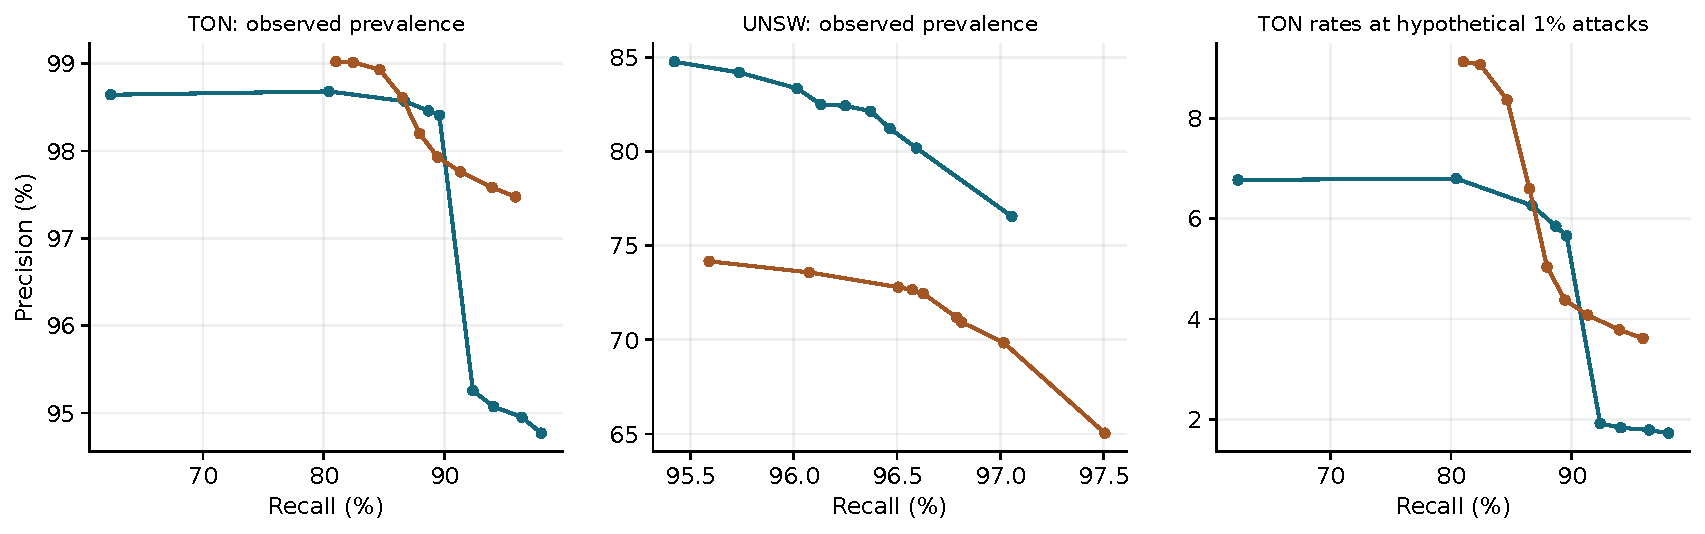
\includegraphics[width=\linewidth]{figures/diagnostic_a_precision_recall.pdf}
\caption{Precision--recall operating points selected by the fixed cost grid. The first two panels use observed class counts. The last panel assumes that TON's class-conditional rates transfer to 1\% attack prevalence. Points are seed means conditional on each capture; they are not pooled adaptive-score PR curves.}
\label{fig:pr}
\Description{Precision--recall operating points selected by the fixed cost grid. The first two panels use observed class counts. The last panel assumes that TON's class-conditional rates transfer to 1\% attack prevalence. Points are seed means conditional on each capture; they are not pooled adaptive-score PR curves.}
\end{figure}



\FloatBarrier
\section{Dataset attributions}
The TON provider requests acknowledgement of the network, telemetry, operating-system, architecture, and related botnet publications \citep{moustafa2021,booij2022,alsaedi2020,moustafa2020windows,moustafa2020linux,moustafa2019dataset,moustafa2019fog,ashraf2021}. The UNSW-NB15 provider's associated papers are also retained \citep{moustafa2015unsw,moustafa2016unsw,moustafa2019geometry,moustafa2017dirichlet,sarhan2021}. Their algorithms are not imported as experimental observations. The input manifests distinguish publisher descriptions from hash-identified public mirrors.
\bibliographystyle{ACM-Reference-Format}\bibliography{references}
\end{document}
